\documentclass[12pt,oneside]{report}

\usepackage[dvipdfmx]{graphicx}
\usepackage{epsfig}
\usepackage{suthesis-2e}
\usepackage{listings}
\usepackage{subfigure}
\lstset{
    language=c,
    basicstyle={\ttfamily},
    breaklines=true,
    columns=[l]{fullflexible},
    lineskip=-0.5zw,
    commentstyle=\textit,
    classoffset=1,
    keywordstyle=\bfseries,
    showstringspaces=false,
    numbers=left,
    stepnumber=1,
    numberstyle=\tiny,
    tabsize=2,
    frame=trbl,
    framesep=5pt
}

\begin{document}

%%%%%%%%%%%%%%%%%%%%%%%%%%%%
% タイトル、学籍番号、著者名
%%%%%%%%%%%%%%%%%%%%%%%%%%%%
\title{学位論文最速文法マスター}
\studentid{1264904}
\author{MAI MAI CUONG}

\univ{Yokohama National University}

%%%%%%%%%%%%%%%%%%%%%%%%%%%%
% 学科名、学位
%%%%%%%%%%%%%%%%%%%%%%%%%%%%
% For B4
\dept{College of Engineering Science} % 工学部
\degree{Bachelor of Engineering} % 学士(工学)

% For M2
\dept{Department of Physics, Electrical and Computer Engineering} % 電気電子ネットワークコース
\degree{Master of Engineering} % 修士(工学)

%%%%%%%%%%%%%%%%%%%%%%%%%%%%
% 提出日(月まで)
%%%%%%%%%%%%%%%%%%%%%%%%%%%%
\submitdate{February 2016}
\copyrightyear{2016}

%%%%%%%%%%%%%%%%%%%%%%%%%%%%
% 指導教官と査読者(B4は指導教官のみ)
%%%%%%%%%%%%%%%%%%%%%%%%%%%%
\principaladviser{KURAMITSU Kimio}
% For M2
\firstreader{HAMAGAMI Tomoki}
\secondreader{HOGE Fuga}

\beforepreface
\tablespagefalse
%%%%%%%%%%%%%%%%%%%%%%%%%%%%
% 概要
%%%%%%%%%%%%%%%%%%%%%%%%%%%%
\prefacesection{Abstract}




%%%%%%%%%%%%%%%%%%%%%%%%%%%%
% 謝辞
%%%%%%%%%%%%%%%%%%%%%%%%%%%%
\prefacesection{Acknowledgements}

本論文は私が横浜国立大学大学院工学府物理情報工学専攻電気電子ネットワークコースに在籍中の研究成果をまとめたものである。
本論文を執筆するにあたり、横浜国立大学工学部電子情報工学科准教授である倉光君郎先生
には、指導教官として研究の方針をご指導頂きました。ここに深く感謝の意を表します。

(stab)

加えて、私の学生生活を長きにわたって見守って下さった私の家族に深く感謝致します。
\afterpreface

\chapter{はじめに}
\label{Introduction}

近年、IoTの発展につれ、様々な機器への組み込みやすさやより高度なパケット処理が必要になった。また、ビックデータ時代になった今は、より高速な構文解析技法が求められている。
そこで、組み込みやすさと高速な処理の面から、FPGA()というデバイスが注目されている。FPGAを用いて、構文解析器を実現する研究がいくつかある。
例えば、研究1では正規表現を使って、FPGA上で構文解析器を作る。正規表現からFPGA合成に必要なHDLファイル、ネットリスト又はコンフィグレーションデータに変換する。しかし、パーサごとに回路を合成しなければならず、手間がかかる。また、開発者にはある程度FPGAの知識が必要である。
また、研究2で文脈自由文法を使ってFPGAでパーサを実現する研究がある。こちらはサブ回路を作ってたくさん並ぶ。ただし、n個のサブ回路がn+1文字しか受理できず、性能的にはよいとは言えない。

FPGAで構文解析器を実現するのは非常に手間がかかる。例えば、ソフトウェア開発と異なり、FPGAの回路では、遅延が発生しているため、開発者は常に遅延時間をいしきしなければならない。また、FPGA開発の際には、合理合成、配線などという段階あり、検証時間が大きい。さらに、新しいプロトコルが続々誕生されている今、それに対応するには、構文解析器を書き換える必要がある。

そこで、本研究の目的は自動生成可能、高速な処理、そして組み込みやすいパーサを実現する。方法としては、解析表現文法からFPGA上でパーサが自動生成する。
ユーザはFPGAの知識が必要なく、文法を定義するpegファイルとテキストを入力するだけで、結果が得られる。



本論文の構成は次の通りである。

第1章:初めに
第2章:FPGA及び解析表現文法PEG
第3章:実装方針
第4章:デザイン
第5章:実装
第6章:実験
第7章:関連研究
第8章:結論


\chapter{関連知識}
この章では、FPGA及びPEGについて説明する。

\section{FPGA}
FPGAとは、ユーザー側で回路を変更することができるデバイスのことである。
FPGA(Field Programmable Gate Array)とは、デジタル回路を構築する大規模集積回路の一種である。通常の集積回路の場合、出荷された回路を変更することができないが、FPGAの場合、出荷された回路も使用者側で任意の論理機能を実装できる。
FPGAは並列度の高い電子回路や機能の専門化によって機能向上した電子回路を容易に構成できる。FPGAは並列処理に擦れており、並列化によって高速化することが可能である。また、ユーザ側が自由に回路を変更することが可能であるため、ある問題に特化した専用回路を作り、性能を向上することができる。

さらに、稼働中の機器のハードウェアも変更できるため、処理の対象や内容に合わせて、状況に応じた回路に書き換えることで、最小限の回路で、多様な処理を実行できる。

一般にFPGA開発の際、ハードウェア記述言語(HDL)が用いられる。本研究では、HDLの一種であるVHDLを使用する。

\section{PEG}
構文解析とは、定義された文法に従ってテキストの構造を解析することである。本研究では、構文解析を実現するために、形式文法を使って、FPGA上でパーサを自動生成する。
形式文法はたくさんの種類がある。例えば、解析表現文法(PEG)や文脈自由文法(CFG)などがある。

本研究では、パーサを構築するために、解析表現文法を使用する。PEGはA <= e というルールの集合である。解析表現は表()にある値と演算子を組み合わせた式である。

PEGのメリットは書きやすく、
強力な表現力をもっている。また、Pactrack を使って線形時間で処理することができる。


\chapter{実装方針}
本研究では、Vitual Machineを採用している。PEGファイルから、実行すべき命令列を生成する。命令セットは以下となる。
命令では、文字の操作の命令と制御用の命令がある。

文字操作の命令はBYTE, SET, ANY がある。こちらの命令は実際に文法定義ファイルの文字とテキストからの文字を比較し、文字を消費するかを判断する。
BYTEは文字リテラルを処理するための命令である。例えば、A =  'a' のPEGである場合、[ BYTE 'a']という命令が生成される。この命令は、現在評価しているテキストの文字が'a'であれば成功でそうでなければ失敗である。
SETは文字クラスを処理するための命令である。例えば、A = [1-9]の場合、[SET [1-9]] という命令が生成される。
ANYは任意の文字を処理するための命令である。例えば、A = . の場合、[ ANY ] という命令がある。
非終端記号はCALL命令を使って、非終端記号の定義されたところにジャンプする。ジャンプする前に、現在命令の次の命令をReturn stackにpushする。RETという命令の時、Return stackからジャンプ先を取得する。
例えば、以下のPEGファイルはこのような命令列が生成される。
Add = Value (+/-) Value
Value = [1-9]

生成された命令列:
Add L1 Call L5
      L2 Set [+/-]
      L3 Call L5
      L4 Ret
Value L5 Set[1-9]
        L6 Ret

まず非終端記号があるため、その非終端記号(L5)へジャンプする。L5にジャンプする前に、L2をReturn stackにpush される。
ここでL5が成功したら、L6に進み、L6はRETであるため、Return stackからジャンプ先をpopされる。先ほどL2をReturn stackにpushされたため、L2にジャンプされる。
次にL2が成功したら、L3に進む。L3でValueを呼び出し、L4をReturn stackにpushされる。
Valueの命令が終ったら、L4に戻る。L4で戻る先がないため、プログラムを終了する。どこから失敗した場合、プログラムが終了される。


ALTはジャンプ先をFail stackにpushする命令である。PEGでは、Option, R~, 選択という演算子があり、どこかの命令が失敗しても、処理が続けることがある。
どこかが失敗した時、Fail stackからジャンプ先を取得する。ALTの使い道はグルーピング、非終端記号、選択を処理する時に使う。具体的に下記に述べる。

Optionを処理するため、2つの方法がある。対象となるOptionは上記の基本要素であれば、その命令と組み合わせて一つの命令として実行する。例えば、'a'?である場合、[ OBYTE 'a']というOptionとBYTEを組み合わせた命令が生成される。
対象となるOption はグルーピングまたは非終端記号の場合、ALTという命令を使って飛び先をstackにpushする。例えば、A = ('a' 'b')? 'c' の場合、'a'を実行する前に、ALTで'c’を評価するための位置をstackにpushする。この
場合、以下の命令列が生成される。

L1 ALT L4 
L2 BYTE 'a'
L3 BYTE 'b'
L4 BYTE 'c'

'a', 'b' でマッチした場合、L2,L3,L4の順に実行される。
一方、例えば'a'で失敗した場合、Failが発生し、stackから飛び先を取得する。先ALTでL4をstackにpushされたため、L4がpopされて、次に実行する命令がL4となる。
Option対象が非終端記号の場合、ALTの後にCALLが実行される。
このように、ALTによってOptionを処理することができる。


0回以上の場合も処理が2つに分かれる。対象がBYTE,SET,ANYの場合、RBYTE, RSET, RANYとして組み合わせた命令を実行する。
対象はグルーピング又は非終端記号の場合、ALT及びJUMPを使って処理する。まずALTでこの処理が終ったときのジャンプ先をFail Stackにpushする。次に、グルーピング・非終端記号の要素を順番に実行し、成功したら、JUMPでグルーピング・非終端記号の最初の要素に戻る。この処理をFailが発生するまで、繰り返される。Failが発生したら、先ALTでpushしたFail stackから、ジャンプ先を取得する。
例えば、以下のPEGはこのような命令列が生成される。
Value = '1' ( '+' '2')*  '+' '3' 

L1 BYTE '1'
L2 ALT L6 
L3 BYTE '+'
L4 BYTE '2'
L5 JUMP L3
L6 BYTE '+'
L7 BYTE '3'
L8 RET

まず、ALTでL6をFail stackにpushする。
つぎに順番にl
L3, L4を実行し、終わったらJUMP命令でL3に戻る。 L3, L4のどこかで失敗するまで、繰り返しが続く。
一方、失敗すると、Fail stackにL6をpopされて、L6が実行される。
1回以上の場合、基本命令と0回以上にみなして実行する。例えば、A = 'a'+ の場合は、[ BYTE 'a']  及び [ RBYTE 'a'] のように命令が生成される。


Choiseの場合、
backtrackを削減するために、選択肢の最初の文字によって、最初にどの選択にするかを決める。この処理をする命令はFIRSTという。複数の選択肢の最初の文字が同じである場合、各選択肢を評価する前に、この選択肢が失敗である場合、別の選択肢に移すためのジャンプ先をALT命令でstackに保存する。
例えば、以下のPEGはこのような命令が生成される。
Value = ('1' '1')/('1' '2')/'3'

L1 FIRST 
	'1' -> L3
	'3' -> L8
	default -> L2
L2 FAIL
L3 BYTE '1'
L4 ALT L7
L5 BYTE '1'
L6 RET
L7 BYTE '2' jump L6
L8 BYTE '3' jump L6

まず、最初の文字によって、jump先が分かれている。
最初の文字が'1'であればL3に、'3'であればL8に、そうでなければL2に移ってFai処理が発生する。
L3にジャンプした場合、まず'1'を消費する。この場合、選択肢が'1' '1'又は'1' '2'の2つがあるため、'1' '1'の選択肢を評価する前に、この選択肢が失敗した場合のジャンプ先をALT命令でFail stackにpushする。もし、この選択肢が成功した場合、L6 のRETで
プログラムを終了させる。一方、失敗した場合、選択肢'1' '2'を評価し、つまりL7が実行される。

否定先読みの場合、処理が2つに分かれる。対象がBYTE,SET,ANYの場合、NBYTE, NSET, NANYとして組み合わせた命令を実行する。
対象はグルーピング又は非終端記号の場合、まずグルーピング・非終端記号を評価する前に、失敗した時のジャンプ先をFail stackにpushする。その後、グルーピング・非終端記号の要素を順序に評価する。どこかで失敗が発生したら、ALTで保存したジャンプ先にジャンプする。この場合は次の解析表現に進むことになる。
ただし、グルーピング・非終端記号が成功した場合、つまり否定先読みが失敗した場合、もしFail処理を発生させるとしたら、ALTで保存されたジャンプ先に飛ぶことになるため、次の解析表現に進んでしまう。
そのため、まずSUCC命令でALTで保存したジャンプ先を消してから、Fail処理を発生させる。
例えば、以下のPEGはこのような命令列が生成される。
Value = !('1'+) [1-9]+
L1 ALT L6
L2 BYTE '1'
L3 RBYTE '1'
L4 SUCC
L5 FAIL
L6 SET [1-9]
L7 RSET [1-9]
L8 RET
 

肯定先読みの場合、対象の表現を順序に評価することになるが、文字を消費しないため、評価する前に、POS命令で今の文字の位置を保存しておく。評価が終ったら、BACK命令で、保存された位置に戻る。
例えば以下のPEGはこのような命令列が生成される。
%Value =/&('1') [1-9]+

L1 POS
L2 BYTE '1'
L3 BACK
L4 SET [1-9]
L5 RSET [1-9]
L6 RET

シーケンスは連続な命令で実行される。


FPGAに情報を渡す前に、前処理としてPEGファイルから命令列を生成する。この処理は本研究室が開発しているNezライブラリを使う。FPGAは命令列を受け取り、テキストを解析する。


\chapter{設計}
\label{Design}
まず、各命令に対応するのサブ回路を作る。
制御部の信号によってどのサブ回路が実行されるのか決められる。

\section{命令用回路}
%\label{k2js}

\subsection{文字操作命令}
文字操作命令はBYTE, SET, ANYがある。

BYTE命令は、テキストの文字と形式文法の文字が一致するかどうかを判断する。BYTE命令用回路の入力はTRG, PEGからの文字、テキストの文字がある。
一致する場合、match信号が'1'となり、逆に一致しない場合はfail信号が'1'となる。Trgがある場合だけ、作動する。Trgがないときはmatch及びfailが'0'となる。
matchが'1'になった場合、次の命令に進む処理をする。failが'1'の場合、Alt命令で保存されたスタックからとび先をもらう。スタックにデータが存在しない場合、プログラムを終了し、パース失敗となる。

ANY命令は、1文字を消費するという命令である。ANY命令用の回路の入力はTRGで、出力はnextchar信号である。TRGがある場合だけ、nextcharが'1'となり、文字を消費する処理を始める。

SET命令用回路の入力は、TRG, PEGからの2の文字、テキス
テキス
テキストの文字がある。文字の範囲か、文字の選択かによって、比較条件が異なる。マッチした場合、matchが'1'となり、マッチしない場合、failが'1'となる。


\subsection{組み合わせ命令}
組み合わせ命令はOption, O個以上、否定先読みをBYTE, SET, ANYを組み合わせた命令である。

Optionの場合、0個マッチしてもよいため、TRGがある場合、matchが'1'となり、この回路からfail信号が発生されない。しかし、文字を消費するかを決めるため、1個マッチした場合、nextcharが'1'となり、文字を消費する。

0個以上の場合、マッチしたら、nextchar信号が'1'となり、文字を消費する。また、nextchar信号がTRGとつながっており、マッチした場合、命令をもう一度実行する(図)。ただし、新たな文字をロードするには、1クロックが必要であるため、nextcharを1クロック遅らせてTRGに入る。このように、マッチしなくなるまで、テキストを消費しながら、回路を動作する。一方、マッチされなくなったら、nextcmd信号が'1'になり、次の命令に進む。

否定先読みの場合、条件を逆にするだけである。


\subsection{その他の命令}

CALL命令用回路は、TRGがあるとき、まずReturn stackに命令がもっている保存用の命令アドレスを追加し、Return stackの先頭をインクリメントする。同時に命令が持っているジャンプ用の命令アドレスをプログラムレジスタにロードする。

ALT命令用回路は、TRGがあるとき、Fail stackに命令が持っている保存用アドレスを追加し、Fail stackの先頭をインクリメントする。

SUCC命令用回路は、TRGがあるとき、Fail stackから先頭の命令アドレスを消し、Fail stackの先頭をデクリメントする。

FAIL命令用回路は、TRGがあるとき、failを'1'となり、Fail処理を発生させる。


\section{制御部}
実効ステップは以下となる。
ステップ1:命令をロード
ステップ2:命令をデコード
ステップ3:命令実行
(図)
ステップ3が終ったら、またステップ1に戻る。





%\begin{figure}[t]
  %  \begin{center}
    %    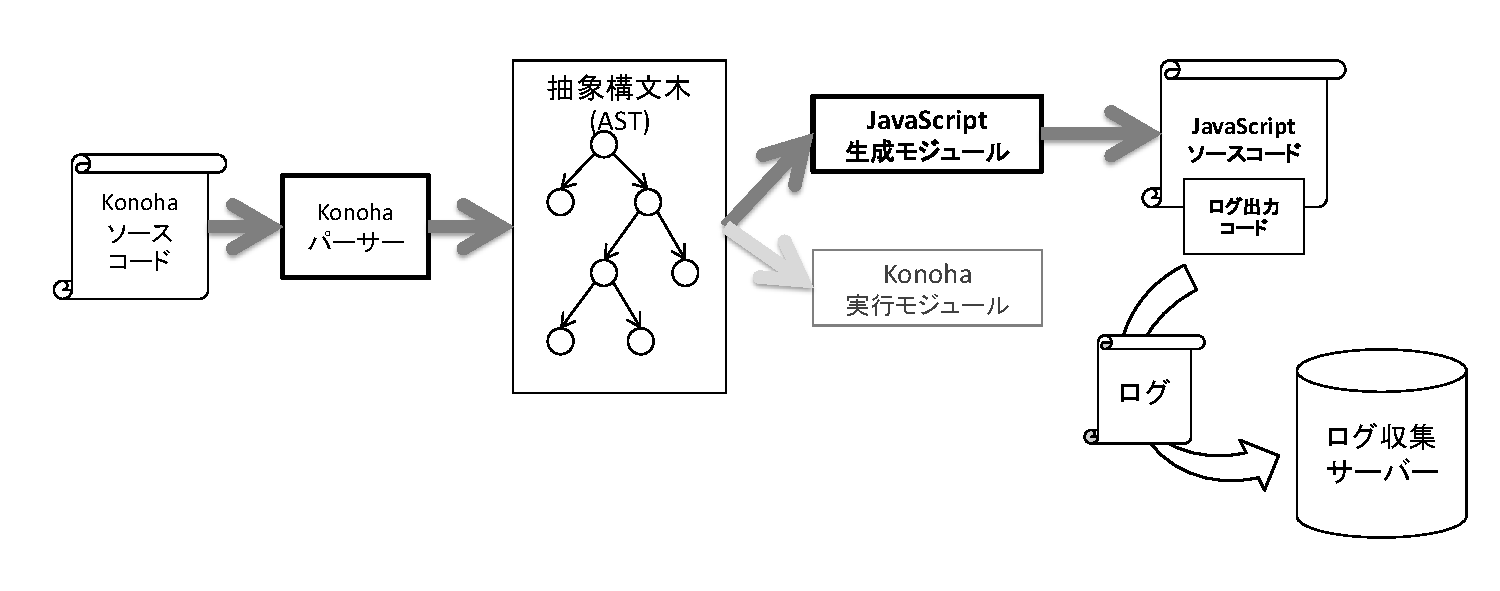
\includegraphics[width=130mm]{./fig/k2js_overview.pdf}
  %      \caption{システムの概要}
   %     \label{fig:k2js_overview}
   % \end{center}
%\end{figure}

%提案手法による処理の流れを図\ref{fig:k2js_overview}に示す。
%KonohaからJavaScriptへのコード変換は、次の手順で行う。
%\begin{enumerate}
%	\item Konohaのソースコードから抽象構文木(AST)を構築する
%	\item JavaScript生成モジュールが、ASTからJavaScriptコードを生成する
%\end{enumerate}

%Konohaではコード生成器はモジュール化されていて、ユーザーが好きなものを選ぶことができる。
%標準では独自のVM(Mini VM)のコードを生成・実行するが、
%モジュールを切り替えることで別のコードを生成可能である。
%Konohaの設計については、文献\cite{Konoha}に詳しいが、特徴としては以下のようなものがある。

%\begin{itemize}
%	\item 拡張可能な文法
%	\item 静的型付け
%	\item クラスベースオブジェクト指向
%	\item 切り替え可能なコード生成器
%\end{itemize}

\chapter{実装}
\label{impr}
%\section{JavaScript生成モジュールの実装}
%本節ではJavaScript生成モジュールの実装において考慮した事柄について述べる。
%\subsection{動的型付けと静的型付け}
%\label{dp}
%Konohaは静的型付けを行う言語であり、変数の型はその変数が宣言された時点で決定する。
%型の異なる値を代入したり、引数に渡したりしているコードは、実行前にエラーが判明するため、
%一般には実行時エラーの少ないプログラミングが可能である。

%\subsection{変数のスコープ}
%\label{scope}
%JavaScriptとKonohaでは変数のスコープが異なっている。
%Konohaはブロックごとにスコープを持つが、JavaScriptでは関数スコープしか存在しない。

\chapter{実験}
\label{exp}

%本手法の評価として、実際に簡単なHTML5アプリケーションをKonohaで記述し、ログを集めることによって、
%端末の性能による実行速度の低下を調べる実験を行った。

%今回の実験では、高性能な環境の例としてPC、性能の低い環境の例としてiPod Touchを用いた。
%各環境の詳細を以下に示す。

%\begin{itemize}
%	\item 高性能環境(PC)
%	\begin{itemize}
%		\item CPU: Intel Core i7-3517U  2.40GHz
%		\item RAM: 4.00GB
%		\item OS: Windows8 Pro
%		\item Browser: 
%	\end{itemize}
%	\item 低性能環境(iPod Touch)
%	\begin{itemize}
%		\item CPU: Apple A4  1.00GHz
%		\item RAM: 256MB
%		\item OS: iOS 6.1
%		\item Browser: 
%	\end{itemize}
%\end{itemize}

%HTML5アプリケーションの例として、Canvasを用いて60フレーム毎秒(60fps)の描画を行う
%アプリケーションを実装し、ログ出力対象に毎フレームの描画関数を指定してコード変換を行った。
%計測回数は100回とした。

%描画関数の平均実行時間は、PCの1.61ミリ秒に対し、iPod Touch環境では31.13ミリ秒と
%約20倍低速になっていた。ここで、60フレーム毎秒で描画する場合、1フレームの実行時間が
%16.6ミリ秒を超えるとフレームレートの低下が発生する。
%ログからiPod Touchにおいてフレームレートが半分の約30fpsに低下することが推測されるが、
%実際にiPod Touch環境ではフレームレートの低下とブラウザの応答速度低下が確認された。

\chapter{関連研究}
\label{RelatedWorks}

%\section{JavaScriptへ変換して実行する言語}
%\label{toJS}
%JavaScriptを用いた開発には問題点も指摘されている。例えば、
%JavaScriptはプロトタイプベースの言語でありクラスが存在しない、
%という問題や、JavaScriptは動的型付け言語であるため、
%一般論として大規模な開発に向かないといった問題である。

%これらの問題を解決するために、近年、開発時には別の言語で記述し、
%JavaScriptへ変換した物を実行するというアプローチがとられるようになっている。
%例として、次のようが言語が挙げられる。
%\begin{itemize}
%	\item CoffeeScript
%	\item Dart
%	\item Haxe
%	\item TypeScript
%	\item JSX
%\end{itemize}
%これらの言語はどれもクラスベースオブジェクト指向言語である。また、この中ではCoffeeScriptは
%動的型付けを採用しているが、その他の言語は静的型付けを採用している。

\chapter{結論}
\label{conc}
%(The great conclusion goes here.)

\bibliographystyle{plain}
\bibliography{mybib.bib}

\end{document}
